\documentclass{article}

\usepackage[main=english,vietnamese]{babel}
\usepackage[T1]{fontenc}
\usepackage[utf8]{inputenc}
\usepackage[sexy]{evan}
\usepackage{matchsticks}
\usepackage{wrapfig}
\usepackage{listings}

\newtheorem{hint}{Hint}

\begin{otherlanguage*}{vietnamese}
\title{Một số bài đề xuất cho Tạp chí Pi}
\end{otherlanguage*}

\author{Nghia Doan}
\date{\today}

\begin{document}

\begin{otherlanguage*}{vietnamese}

\maketitle

\begin{example*}[Bài 1]
    Chứng minh rằng tồn tại vô số số nguyên dương sao cho trung bình cộng và trung bình nhân của các ước số của số đó đều là số nguyên.
\end{example*}

\begin{proof} (\textit{Bài 4, Lớp 10, Kazahstan Math Olympiad 2011})
    Giả sử $p$ là số nguyên tố bất kỳ dạng $3k+1.$ $p^2$ có ba ước số là 1, $p$, và $p^2.$
    Trung bình cộng và trung bình nhân của các ước số này có thể biểu diễn như sau:
    \[
        \sqrt[3]{1 \cdot p \cdot p^2} = p,\ \frac{1+p+p^2}{3} = \frac{1 + (3k+1) + (3k+1)^2}{3} = 3k^2 + 3k + 1.
    \]

    Dễ nhận thấy cả hai đều là số nguyên. Tồn tại vô số số nguyên tố dạng $p=3k+1,$ do đó tồn tại vô số nguyên dương $p^2$ thoả mmãn điều kiện đề bài.
\end{proof}

\newpage

\begin{example*}[Bài 2]
    $n$ là số nguyên dương, $n \ge 3.$ $a_1, a_2, \ldots, a_n$ là các số thực dương sao cho:
    \[
        \frac{1}{1+a_1^4} + \frac{1}{1+a_2^4} + \cdots \frac{1}{1+a_n^4} = 1.
    \]

    Chứng minh rằng:
    \[
        a_1 a_2 \cdots a_n \ge (n-1)^{\frac{n}{4}}.
    \]
\end{example*}

\begin{proof} (\textit{Bài 5, Macedonia National Olympiad 2016})
    Với $i=1,2, \ldots, n,$ đặt $x_i = \dfrac{1}{1+a_i^4},$ khi đó
    \[
        x_1 + x_2 + \cdots + x_n = 1\ \text{và}\  a_i = \left( \frac{1-x_i}{x_i} \right)^{\frac{1}{4}},\ i=1,2, \ldots, n.
    \]

    Do đó,
    \[
        a_1^4 = \frac{x_2 + x_3 + \cdots + x_n}{x_1},\ a_2^4= \frac{x_1 + x_3 + \cdots + x_n}{x_2}, \ldots,\ a_n^4= \frac{x_1 + x_2 + \cdots + x_{n-1}}{x_n}.
    \]

    Áp dụng bất đẳng thức trung bình cộng - trung bình nhân (AM-GM), ta có:
    \[
        \begin{cases}
            &x_2 + x_3 + \cdots + x_n \ge (n-1)\sqrt[n-1]{x_2x_3 \cdots x_n}\\
            &x_1 + x_3 + \cdots + x_n \ge (n-1)\sqrt[n-1]{x_1x_3 \cdots x_n}\\
            &\ldots\\
            &x_1 + x_2 + \cdots + x_{n-1} \ge (n-1)\sqrt[n-1]{x_1x_2 \cdots x_{n-1}}\\
        \end{cases}
    \]

    Vì vậy,
    \[
        \begin{aligned}
            &(a_1 a_2 \cdots a_n) ^ 4 = \frac{x_2 + x_3 + \cdots + x_n}{x_1} \cdot \frac{x_1 + x_3 + \cdots + x_n}{x_2} \cdots \frac{x_1 + x_2 + \cdots + x_{n-1}}{x_n}\\
            &\ge (n-1)^n \frac{\sqrt[n-1]{x_2x_3 \cdots x_n}\sqrt[n-1]{x_1x_3 \cdots x_n} \cdots \sqrt[n-1]{x_1x_2 \cdots x_{n-1}}}{x_1x_2 \cdots x_n}
            = (n-1)^n\\
        \end{aligned}
    \]

    Lấy căn bậc bốn cho hai vế: $\boxed{a_1 a_2 \cdots a_n \ge (n-1)^{\frac{n}{4}}.}$
\end{proof}

\newpage

\begin{example*}[Bài 3]
    Cho $k$ là một số nguyên dương.

    Hai người chơi A và B chơi một trò chơi trên một lưới vô hạn được tạo thành từ các lục giác đều.
    Hai hình lục giác trống liền kề trong lưới là hai ô có chung một cạnh. 

    Ban đầu tất cả các ô lưới đều trống. A và B lần lượt thay nhau đi. A đi trước.
    Trong nước đi của mình, A có thể chọn hai hình lục giác trống liền kề trong lưới và đặt một viên sỏi vào mỗi một trong hai hình lục giác đó.
    Trong nước đi của mình, B có thể chọn bất kỳ viên sỏi nào đang ở trên lưới và bỏ nó ra ngoài.
    Nếu tại bất kỳ thời điểm nào có $k$ ô lưới liên tiếp trên cùng một dòng mà tất cả đều chứa sỏi thì A sẽ thắng.
    
    Tìm giá trị nhỏ nhất của $k$ mà A không thể thắng trong một số hữu hạn nước đi, hoặc chứng minh rằng không tồn tại giá trị nhỏ nhất đó.
\end{example*}

\begin{proof} (\textit{Bài 5, Ngày 2, USAJMO 2014})
    Đầu tiên, ta chứng minh rằng A  không thể thắng trong một số hữu hạn nước đi nếu $k=6.$
    Tô lưới lục giác đều bằng hai màu trắng và nâu như hình bên dưới.

    \begin{center}
        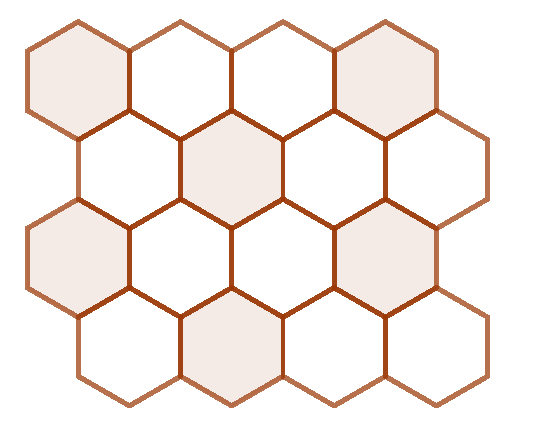
\includegraphics[width=6cm]{./svg/pdf/pi-2024-1-p3.pdf}
    \end{center}

    Dễ thấy rằng sau mỗi bước A chỉ có thể có đúng một viên sỏi trên ô màu nâu.
    Chiến thuật của B là lấy viên sỏi trên ô màu nâu đó. Như vậy số viên sỏi trên các ô màu nâu mà A có thể có không vượt quá một.
    Trong khi đó, sáu ô lưới liên tiếp trên cùng một dòng luôn chứa ít nhất hai ô màu nâu.
    Do đó A không thể thắng được.

    Bây giờ ta sẽ chứng minh A có chiến thuật để thắng với $k=5.$
    
    Ở bước đầu tiên, A đặt lên lưới hai viên sỏi ở hai ô liên tiếp, xem hình dưới bên trái. Màu nâu để đánh dấu là ô có chứa sỏi.
    B chọn và bỏ một viên ra ngoài. Sau hai bước đầu tiên, trên lưới có đúng một viên sỏi,
    xem hình dưới bên phải: chỉ có một ô màu nâu (còn chứa sỏi), ô màu trắng không chứa sỏi.

    \begin{center}
        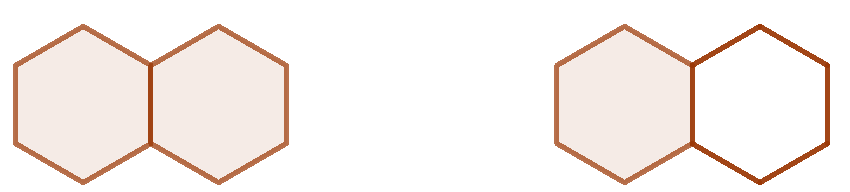
\includegraphics[width=6cm]{./svg/pdf/pi-2024-1-p3-1-2.pdf}
    \end{center}

\newpage

    Trong bước ba, A có thể đặt hai viên sỏi tạo thành một hàng với viên còn lại ở bước hai, xem hình dưới bên trái.
    B chọn và bỏ một viên ra ngoài. Trên lưới còn hai viên sỏi liền kề hoặc trên cùng một hàng và cách nhau một ô, xem hình dưới bên phải. 

    \begin{center}
        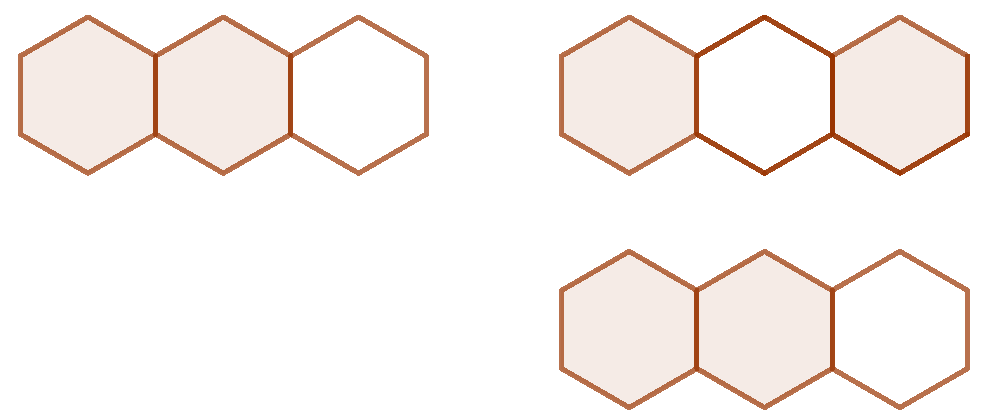
\includegraphics[width=6cm]{./svg/pdf/pi-2024-1-p3-3-4.pdf}
    \end{center}

    Ở bước năm, A có thể đặt hai viên sỏi tạo thành ba viên trên cùng hàng và viên thứ tư liền kề với hai viên đầu tiên trong hàng, xem hình bên dưới thứ nhất từ trái sang.
    
    Lúc này B có ba chọn lựa cho bước thứ sáu: (6a) B bỏ viên dưới cùng (ở hàng thứ hai), xem hình thứ hai, A sẽ thắng trong bước bảy khi đặt hai viên vào cùng hàng đã có sẵn ba viên.
    hoặc (6b) - (6c)- (6d): B bỏ một viên ở hàng trên, xem hai ví dụ ở hai hình thứ ba và thứ tư.

    \begin{center}
        \begin{minipage}[t]{6.5cm}
            \begin{center}
                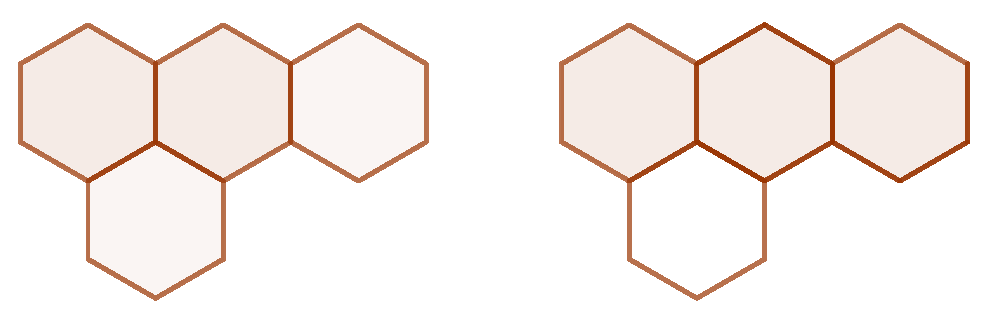
\includegraphics[width=6cm]{./svg/pdf/pi-2024-1-p3-5-6a.pdf}
            \end{center}
        \end{minipage}
        \qquad
        \begin{minipage}[t]{6.5cm}
            \centering
            \begin{center}
                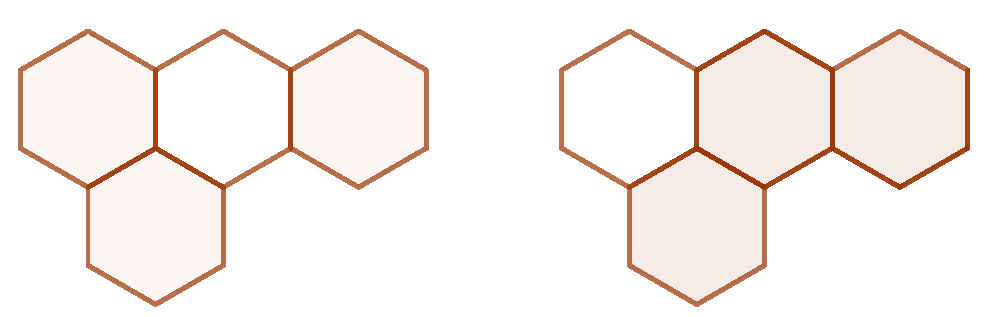
\includegraphics[width=6cm]{./svg/pdf/pi-2024-1-p3-6b-6c.pdf}
            \end{center}
        \end{minipage}
    \end{center}
   
    Ở bước bảy, từ lựa chọn của B theo (6b) - (6c)- (6d), A sẽ thêm hai viên vào một trong hai bên để tạo thành hình bên dưới thứ nhất từ bên trái.
    
    Vào bước tám, B có thể: (8a) bỏ một trong hai viên ngoài cùng bên trái hoặc bên phải, xem hình bên dưới thứ hai từ bên trái;
    hoặc (8b) bỏ viên ở giữa, xem hình bên dưới thứ ba từ bên trái;
    
    \begin{center}
        \centering
        \begin{minipage}[t]{6.5cm}
            \begin{center}
                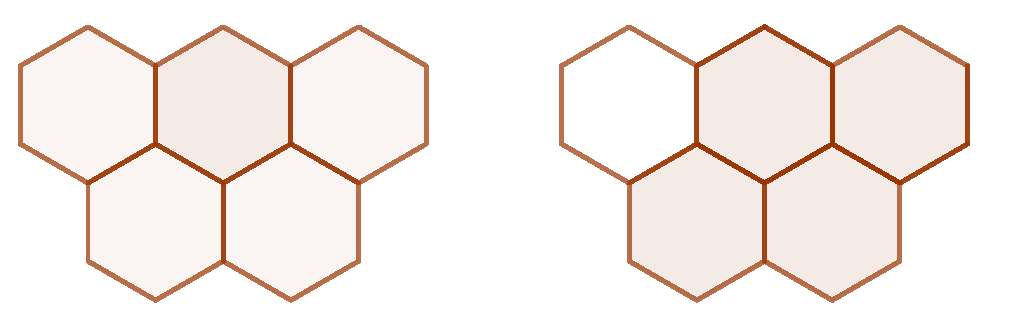
\includegraphics[width=6.5cm]{./svg/pdf/pi-2024-1-p3-7-8a.pdf}
            \end{center}
        \end{minipage}
        \qquad
        \begin{minipage}[t]{3cm}
            \raggedleft
            \begin{center}
                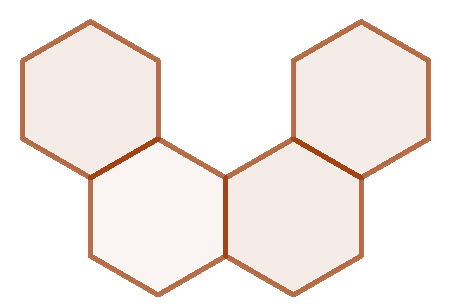
\includegraphics[width=3cm]{./svg/pdf/pi-2024-1-p3-8b.pdf}
            \end{center}
        \end{minipage}
    \end{center}

    Ở bước chín, nếu B chọn (8a), A sẽ thêm hai viên vào một trong hai bên để tạo thành hai hàng, mỗi hàng có ba viên liền kề, xem hình dưới bên trái.
    Bất kể B chọn gì ở bước mười, A sẽ thắng ở bước mười một.

    Nếu B chọn (8b) trong bước chín này, A sẽ thêm hai viên vào để tạo thành hình dưới bên phải.

    \begin{center}
        \centering
        \begin{minipage}[t]{3.5cm}
            \begin{center}
                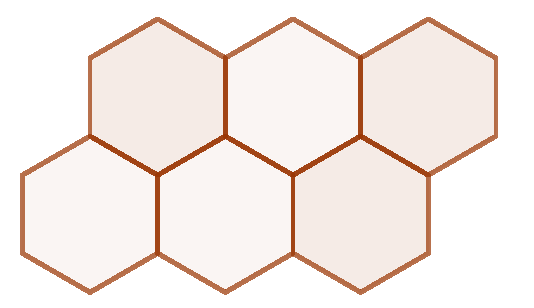
\includegraphics[width=3.5cm]{./svg/pdf/pi-2024-1-p3-9a.pdf}
            \end{center}
        \end{minipage}
        \qquad
        \begin{minipage}[t]{4cm}
            \begin{center}
                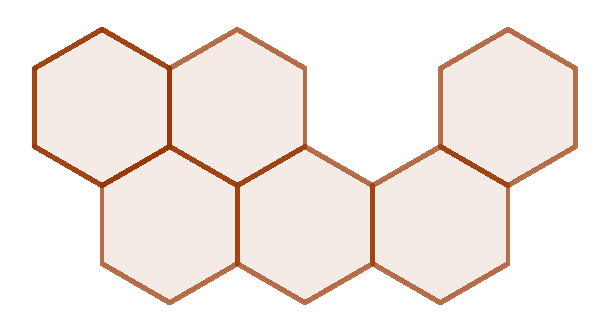
\includegraphics[width=4cm]{./svg/pdf/pi-2024-1-p3-9b.pdf}
            \end{center}
        \end{minipage}
    \end{center}

    Ở bước mười, B có ba lựa chọn, xem hình bên dưới.

    \begin{center}
        \centering
        \begin{minipage}[t]{4cm}
            \begin{center}
                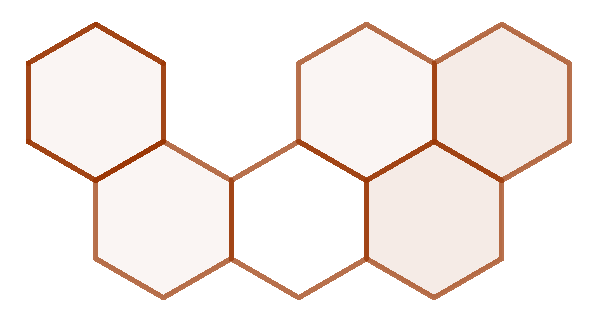
\includegraphics[width=4cm]{./svg/pdf/pi-2024-1-p3-10a.pdf}
            \end{center}
        \end{minipage}
        \quad
        \begin{minipage}[t]{4cm}
            \begin{center}
                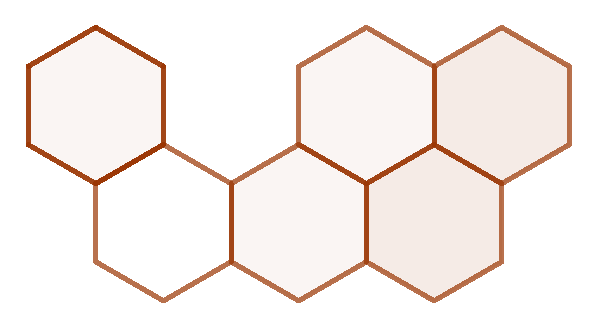
\includegraphics[width=4cm]{./svg/pdf/pi-2024-1-p3-10b.pdf}
            \end{center}
        \end{minipage}
        \qquad
        \begin{minipage}[t]{4cm}
            \begin{center}
                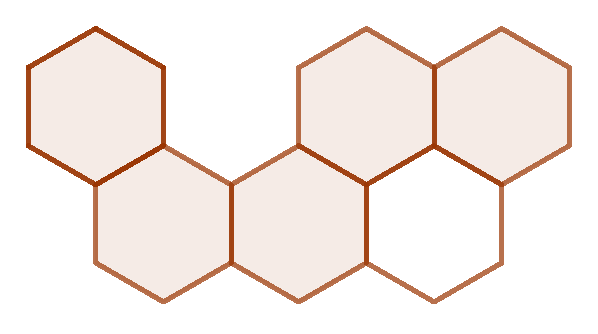
\includegraphics[width=4cm]{./svg/pdf/pi-2024-1-p3-10c.pdf}
            \end{center}
        \end{minipage}
    \end{center}

    Ở bước mười một, tuỳ theo lựa chọn của B, A có thể thêm vào hai viên để tạo nên một trong hai tình huống, xem hình bên dưới.

    \begin{center}
        \centering
        \begin{minipage}[t]{4cm}
            \begin{center}
                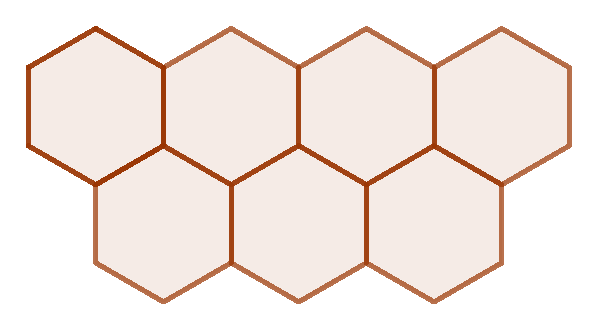
\includegraphics[width=4cm]{./svg/pdf/pi-2024-1-p3-11a.pdf}
            \end{center}
        \end{minipage}
        \qquad
        \begin{minipage}[t]{4.8cm}
            \begin{center}
                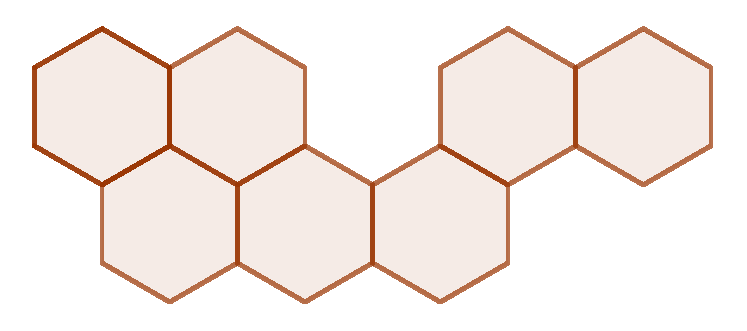
\includegraphics[width=4.8cm]{./svg/pdf/pi-2024-1-p3-11b.pdf}
            \end{center}
        \end{minipage}
    \end{center}

    Dễ thấy rằng A sẽ thắng ở bước mười ba, bất kể B bỏ đi viên sỏi nào ở bước mười hai.

    Như vậy, giá trị nhỏ nhất của $k$ mà A không thể thắng trong một số hữu hạn nước đi là $\boxed{6.}$
\end{proof}

\newpage

\begin{example*}[Bài 4]
    $ABC$ là một tam giác nhọn. $D$ là điểm giữa của cung $BC$ không chứa $A$ trên đường tròn ngoại tiếp tam giác $ABC.$
    $E$ và $F$ là hai điểm đối xứng với $D$ lần lượt qua đoạn thẳng $BC$ và tâm đường tròn ngoại tiếp.
    $K$ là điểm giữa đoạn $AE.$ Chứng minh rằng:
    \begin{itemize}[topsep=0pt, partopsep=0pt, itemsep=0pt]
        \ii Đường tròn đi qua ba trung điểm $M, N,$ và $L$ của các cạnh $BC, CA,$ và $AB$ cũng đi qua điểm $K.$
        \ii Đường thẳng đi qua hai điểm $K$ và $M$ vuông góc với đoạn thẳng $AF.$
    \end{itemize} 
\end{example*}

\begin{center}
    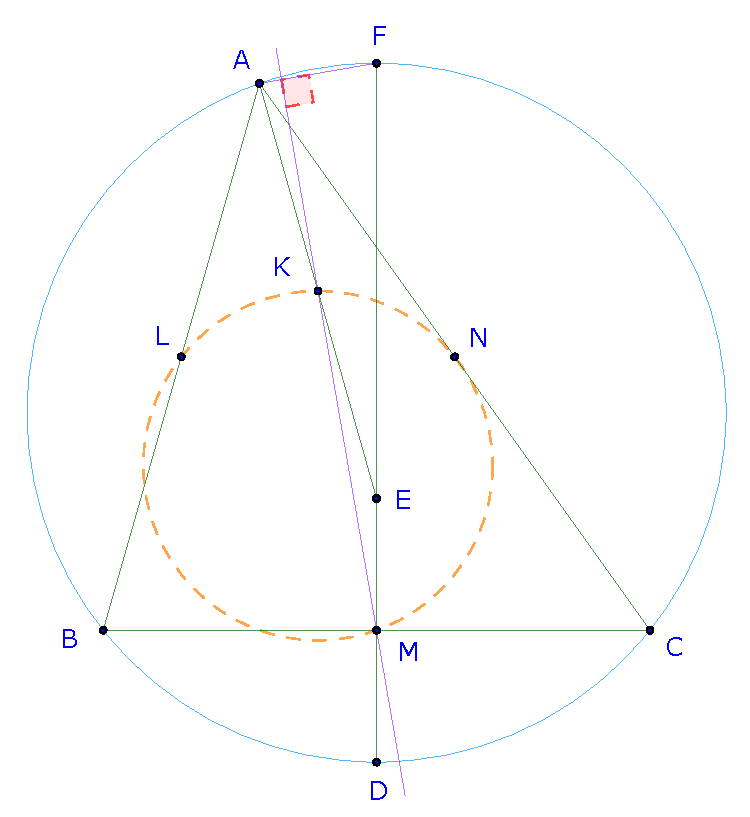
\includegraphics[width=10cm]{./svg/pdf/pi-2024-1-p4.pdf}
\end{center}

\begin{proof} (\textit{Bài 1, Balkan Math Olympiad 1999})
    Ta có $LM \parallel AC,$ $MN \parallel AB,$ do đó: $\angle LMN = \angle LAN = \angle BAC.$

    Do $K$ là trung điểm $AE,$ nên $LK \parallel BE$ và $KN \parallel CE,$ vì thế $\angle LKN = \angle BEC.$
    $E$ là điểm đối xứng với $D$ qua $BC$ nên $\angle BEC = \angle BDC.$

    Tổng hai góc đối diện $\angle LKN$ và $\angle LMN$ trong tứ giác $MNKL$ là:
    \[
        \angle LKN + \angle LMN = \angle BDC + \angle BAC = 180\dg,
    \]
    do đó $MNKL$ là tứ giác nội tiếp, và $K$ nằm trên đường tròn đi qua ba điểm $M, N,$ và $L.$

    $D$ là điểm giữa cung $BC,$ cho nên $BD = DC.$ Vi $E$ là điểm đối xứng với $D$ qua $BC$ nên $BDCE$ là hình thoi.
    Vì vậy $M$ là trung điểm của $DE.$ Do $K$ là trung điểm $AE$ nên $KM \parallel AD.$
    
    $DF$ là đường kính của đường tròn ngoại tiếp tam giác $ABC,$ do đó $AD \perp AF.$
    Từ đó suy ra $KM \perp AF.$
\end{proof}

\end{otherlanguage*}

\end{document}